%\introduction command is provided as a convenience.
%if you want special chapter formatting, you'll probably want to avoid using it altogether
		
\chapter*{Introduction}
    \addcontentsline{toc}{chapter}{Introduction}
		\chaptermark{Introduction}
		\markboth{Introduction}{Introduction}
% The three lines above are to make sure that the headers are right, that the intro gets included in the table of contents, and that it doesn't get numbered 1 so that chapter one is 1.
\begin{quote}
	    ``While the founding fathers agonized over the question `particle' or `wave', de Broglie in 1925 proposed the obvious answer `particle' and `wave'... [t]his idea seems to me so natural and simple, to resolve the wave-particle dilemma in such a clear and ordinary way, that it is a great mystery to me that it was so generally ignored." -J. S. Bell
	    \end{quote}
	    
	    %"Six Possible Worlds of Quantum Mechanics" (1986), included in Speakable and Unspeakable in Quantum Mechanics (1987), p. 191

	    
	    %``For those who are not shocked when they first come across quantum theory cannot possibly have understood it." - Niels Bohr.


Quantum mechanics is perhaps one of the most counter-intuitive scientific theories in the history of the scientific method. At the atomic level, where quantum effects dominate, the laws that seem to govern our everyday world are no longer relevant. Determinism, the idea that every effect has a cause, is replaced with the idea that every action is probabilistic. A particle cannot be described by precise coordinates; instead, it is described using a wavefunction which provides a range of possible locations with associated probabilities. This probabilistic interpretation of quantum mechanics is known as the Copenhagen interpretation, and represents the most common form of rationalizing the radical, experimental observations of quantum mechanics. 

In 2005, Couder et al. showed that oil drops bouncing on a vertically vibrated fluid bath exhibit properties analogous to the paradoxical properties previously seen only at the quantum scale\rf{Couder2005b}.  The system operates at the macroscale, meaning that it is governed by the more ``intuitive" classical laws, but still behaves \textit{like} a quantum system. The accessibility of this experiment allows us to observe fundamental, ``quantum"-like phenomena in a way that is impossible at the nanoscale. For example, in quantum mechanics, one can never know the position \textit{and} the velocity of a particle, simply because it can never \textit{have} a perfectly defined position and velocity. In this experiment, however, the ``particle" can be easily seen at all times, so both its position and velocity can be easily tracked. 

    The behavior of the droplet system seems to agree with a theory of quantum mechanics proposed by Louis de Broglie in 1923 known as pilot-wave theory \rf{dB23,dB87}. Unlike the probabilistic viewpoint subscribed to by adherents of the Copenhagen interpretation, de Broglie's model asserts that the particle \textit{has} a precise location, and that the particle is pushed by a guiding or ``pilot" wave. The theory was extended by David Bohm in 1952 \rf{Bohm1952a,Bohm1952b}, but never caught on because it gained ``realism" (the idea that a particle is well defined at all times) at the expense of ``locality" (the idea of a universal speed limit where nothing, including information, can travel faster than the speed of light required by special relativity); a trade that is generally considered unfavorable by physicists.\footnote{The Copenhagen interpretation of quantum mechanics, by the way, is non-realist but local.} 
    
    De Broglie's original theory is underdeveloped, having remained relatively obscure for the better part of the last century. Since the predictions of the Copenhagen interpretation and de Broglie's theory are similar, experiments have done little to clarify the debate. As a result, the more developed Copenhagen school of thought holds its place as \textit{the} interpretation of quantum phenomena. 
    
     After taking a course in quantum mechanics, I found it difficult to truly believe some of the associated implications of the Copenhagen interpretation. I was seduced by some of the more obscure quantum methodologies that promised salvation from indeterminism and non-realism (such as Bohm or de Broglie's theories), and it was difficult from me to resist the opportunity to investigate analogs of these methodologies in an experimental setting. The bouncing droplet system, which serves as a hydrodynamic quantum analog and forms the backbone of this thesis, is introduced below. 
    
%Particle-wave association on a fluid interface (Protiere 2006).
	    \subsection*{Bouncing Droplets}
	    Though it had been observed for at least a century, the phenomena of droplets bouncing on a fluid bath was first explained by Jearl Walker in 1978\rf{Walker}. The investigations began with a simple droplet of water falling onto a bath of water and remaining just a second too long before coalescence.\footnote{It is often reported that this occurs in coffeemakers, as the coffee drips into the pot.} Walker discovered that by adding detergent to the water and vibrating the bath, he could extend the lifetime of the droplets from fractions of a second to several minutes. These droplets bounce at frequencies of around 50 Hz (50 bounces per second) and are very small, with a diameters of a millimeter or less. These two factors make it difficult to observe even the main mechanisms that drive the behavior. A key insight by Walker was that by flashing a strobe light at a frequency slightly slower than the rate of vibration of the bath, he could observe the droplet bouncing as if in slow motion.
	    
\begin{figure}[h!]
	\centering
	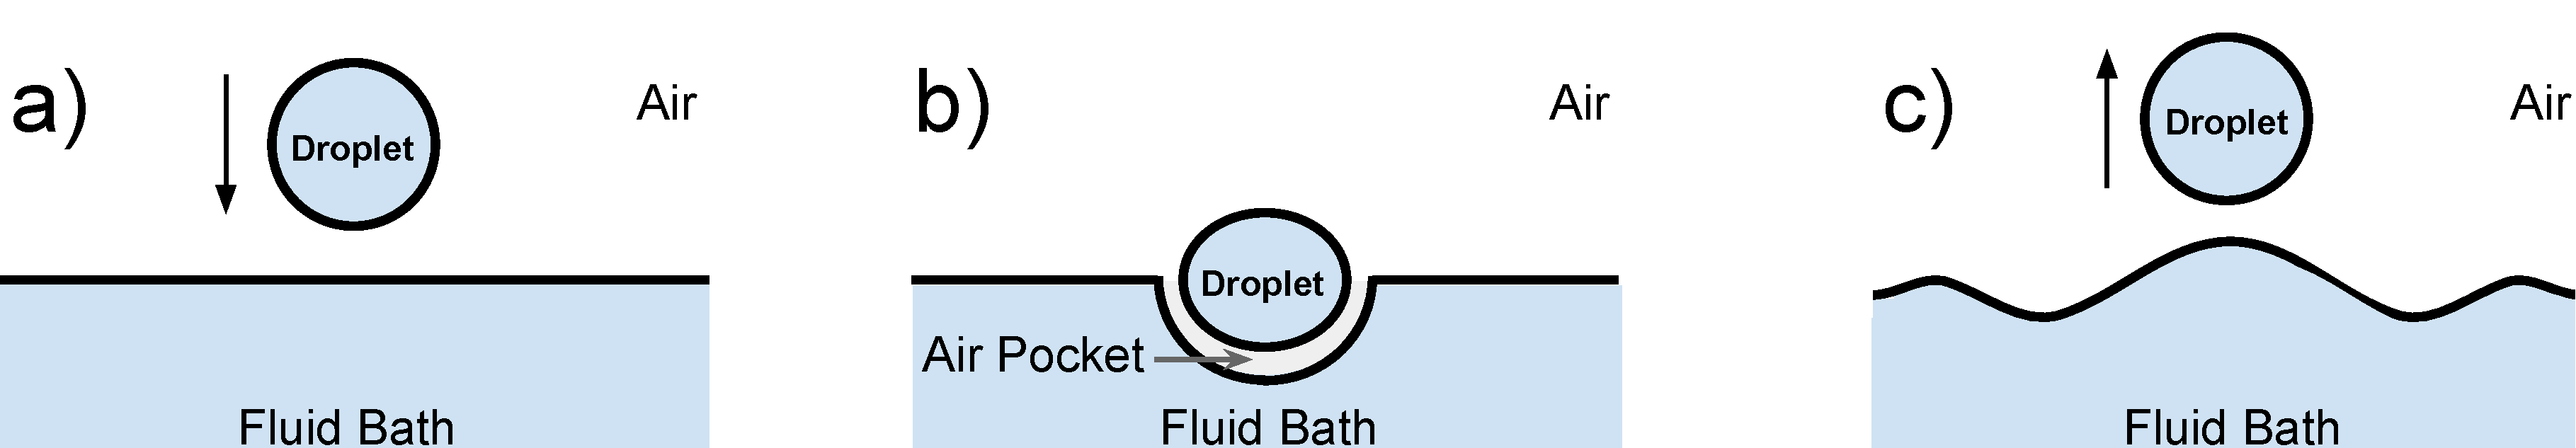
\includegraphics[scale=0.25]{BouncingDroplet.pdf}
	\caption{A depiction of a droplet bouncing on a bath of the same fluid. (a) A droplet falls onto a fluid bath. (b) A film of air gets trapped underneath the droplet. (c) The droplet bounces back up off of the cushion of air leaving behind waves that propagate radially.}
	\label{bounce}
\end{figure}
	    
	    Walker found that a trapped film of air kept the droplet and the bath from touching, as shown in \refFig{bounce}. That is, the droplet is bouncing on a layer of air that is being pushed out from under the droplet, but because the bounce happens so quickly, the fluid droplet and the fluid bath never touch. Walker concluded that the leakage rate of this trapped pocket of air depends on three factors: the surface tension of the fluid in the bath, the viscosity of the droplet and the fluid bath, and the viscosity of air. He found that the bath must be of uniform surface tension and free from floating particulate matter, since both could lead to coalescence. Higher viscosity fluids led to longer droplet lifetimes, since more viscous fluids make it more difficult for air to escape the gap between the drop and the bath. Finally, adjusting the frequency and the amplitudes of the vibrations also affected droplet lifetime.\footnote{Reedie Andrew Case ('92) wrote his thesis ``Oil on Troubled Water: The Extension of Floating Drop Lifetimes Due to Interface Vibration" where he looked at droplet lifetime as a function of vibrational frequency.}   
	     
	    More recent research showed that droplets of fluids like silicone oil can bounce indefinitely on a vibrating bath\rf{Couder2005a}. The long lifetime occurs not only because silicone oil has a high viscosity, but also because it has a \textit{low} surface tension. A low surface tension is beneficial because it makes the oil bath relatively immune to surfactants (e.g. detergent) or contamination that would otherwise make the surface tension nonuniform and lead the drop to coalescence. 

\subsection*{Faraday Waves}
	    The behavior of a fluid in a vertically vibrated bath can be controlled by adjusting the amplitude or the frequency of the vibration. Depending on a variety of factors (size of bath, fluid in bath, etc.) each system has a specific amplitude (given a specific frequency), which if surpassed, will produce standing surface waves called Faraday waves\rf{Faraday}.\footnote{Faraday waves were not actually discovered by Michael Faraday; in the footnotes of his paper he cites that they were first observed by Oersted, Wheatstone, Weber, and others. Faraday was just the first to study their behavior in detail.}~\footnote{Another Reed thesis, this one titled ``Good Vibrations: A Visual Exploration of Faraday Waves" by Alison Saunders empirically tested the mathematical Faraday wave model. } A vibrating bath below this critical amplitude, also known as the Faraday threshold, will have a quiescent surface. A bath driven at an amplitude greater than the Faraday threshold will have a turbulent surface with ripples and waves. An example of Faraday waves is shown in \refFig{faraday waves}. Adjusting the frequency above the Faraday threshold will change the size and shape of the Faraday waves. Note that Faraday waves can be created either by increasing the driving amplitude above a critical level, or adjusting frequency.	    
	    \begin{figure}[h!]
	\centering
	\includegraphics[scale=0.06]{Faraday.JPG}
	\caption{A picture of Faraday waves in a dish of water at $80~\mathrm{Hz}$.}
	\label{faraday waves}
\end{figure}

\subsection*{Walking Droplets}
	    
	A bouncing droplet will bounce differently depending on the frequency and amplitude of the vertical vibrations. If the parameters are set just below the Faraday instability, a curious motion arises: the droplet seems to ``walk" across the surface of the oil. The droplet is being pushed by its own ripples, a dual effort in which neither can exist without the other. In essence, the walker is both a particle and a wave; a conjunction reminiscent of the quantum scale. 
	  
\begin{figure}[h!]
	\centering
	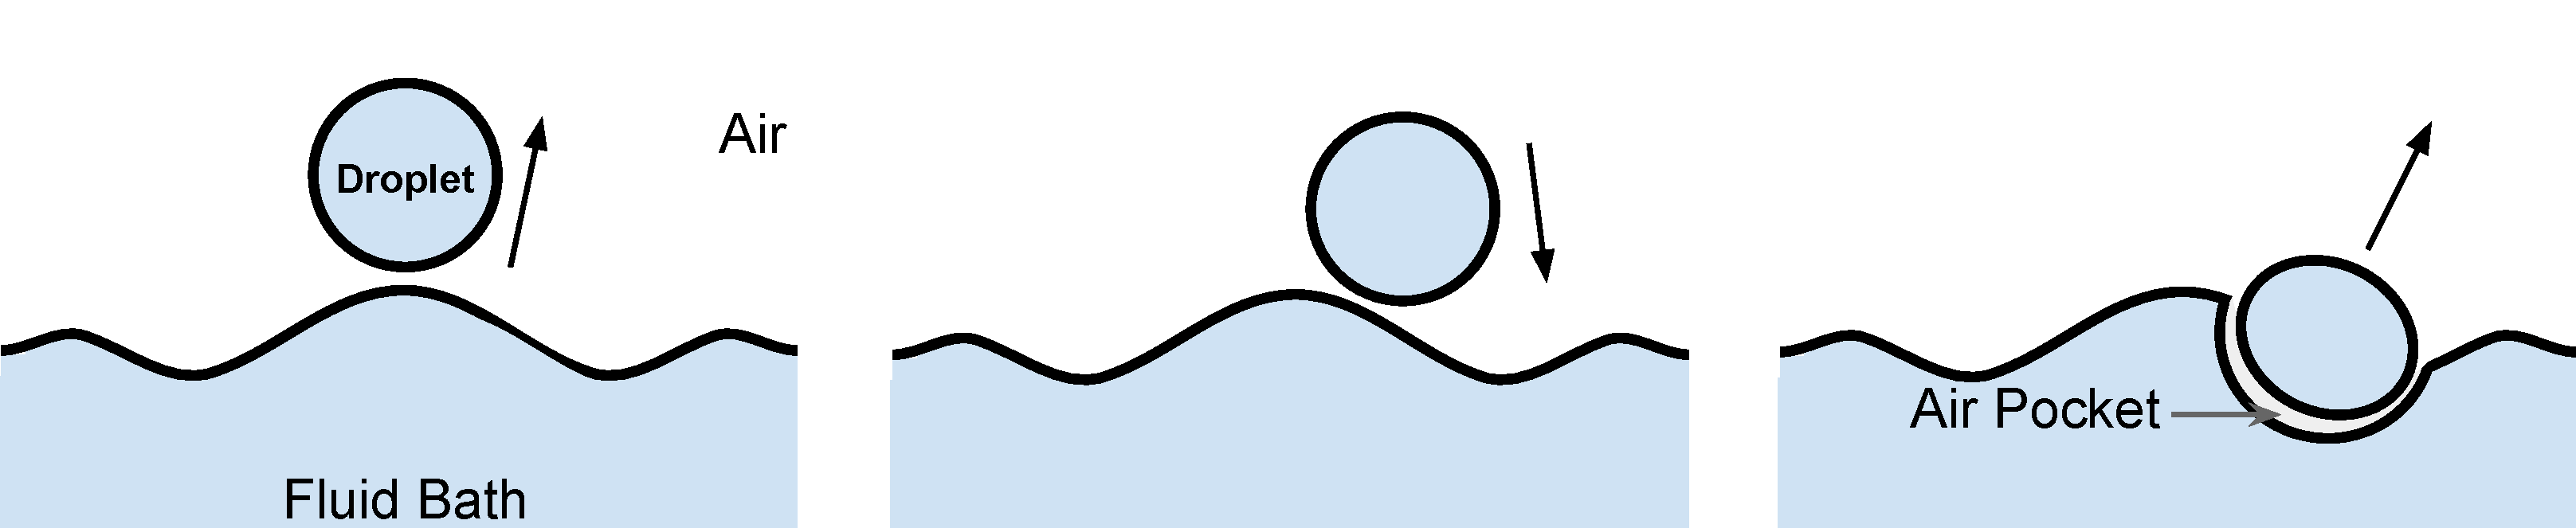
\includegraphics[scale=0.28]{Walking.pdf}
	\caption{A depiction of a droplet walking across a bath of the same fluid.}
	\label{bounce}
\end{figure}
	    
	  
\subsection*{Overview}	  
	  
	Recently, two main groups have been investigating the properties of this unique system. A group at Laboratoire Mati\`{e}re et Syst\`{e}mes Complexes (MSC) in Paris, France, headed by Yves Couder was the first to uncover some of the inherently ``quantum"-like behavior of bouncing droplets, in 2005~\cite{Couder2005b}. Since 2010, John Bush's group at MIT have created a mathematical model and performed their own investigations of the walker system. Couder, Bush, and others have shown that this system can reproduce double-slit single-particle interference \rf{double-slit}, tunneling \rf{tunneling}, quantized orbits \rf{Oza2014}, and many other ``quantum"-like effects \rf{pilot-wave}. 
		
	This thesis documents an experimental investigation into the ``tunneling" behavior of this bouncing droplet system. In this setting, tunneling occurs when the droplet interacts with a submerged barrier. Only one other study looks at this aspect~\cite{tunneling}, but falls short of completely examining the tunneling behavior, focusing on the effect of barrier width and not examining barrier height. I hope to add to the body of work in this subfield by studying how barrier height affects probability of tunneling.   
	
	This thesis is divided into three main chapters. \textbf{Chapter 1} describes the hydrodynamic quantum analog along with a brief survey of the relevant literature. \textbf{Chapter 2} describes the experimental design and explains the setup and the data acquisition procedures. \textbf{Chapter 3} presents the data from my experiments. Finally, the \textbf{Conclusion} highlights the results, summarizes the limitations, and suggests avenues for future study. 